% !TEX root =  ../notes.tex
\chapter{Robot Dynamic Modeling (review)}                
\section{Modeling Robot Manipulators}
                    A set of rigid bodies (called links), connected by joints (see Fig.~\ref{fig:manipulator}). 
                    The most common types of joints are:
                    \begin{enumerate}
                        \item revolute: allow rotation around a fixed axis;
                        \item prismatic: allow translation along a fixed axis.
                    \end{enumerate}
                    Joints are typically actuated by a \underline{motor} and a \underline{transmission system}, e.g. gearbox, cable-driven transmission, pulleys.
                    We typically need a transmission system because we do not want to have the motor located at the joint (such as at the wrist joint, which is far from the base and would result in inefficient motions), but we want the motor as close as possible to the robot base.
                    Moreover, the problem with almost all actuators/motors is that they provide high velocities and small torques.
                    On robots we need the opposite: high torques and small velocities: with a gear-box (gear ratio) we are able to reduce the velocity and get a higher torque. 
                    
                    The positions and angles of the $n$ joints of a robot are encoded by the variables $q_{i} \, \, \, \, \forall i = 0, .., n-1$.
                    These \textbf{joint coordinates} can be collected in an $n$-dimensional vector $q$.
                    \begin{figure}[t]    
                        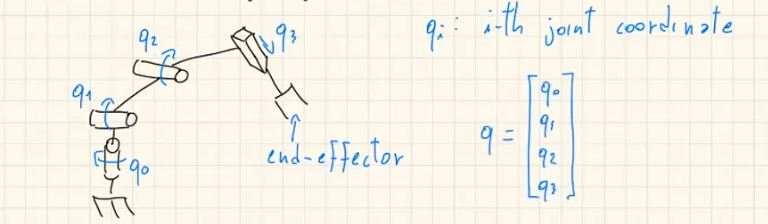
\includegraphics[width = \textwidth, height = 6cm]{robotManipulatorModel.JPG}
                        \caption{Robot Manipulator Model}
                        \label{fig:manipulator}
                    \end{figure}
                    
\subsection{Homogeneous Transformations}
                    When working with a robot very often we are not interested in the joint angles, but in the position and orientation (pose) of the end-effector (e.e.), which is where the robot behavior can be more easily specified.
                    To define the pose of the e.e. we need a reference frame $RF_0$ (fixed) and a body (rigid) (with reference frame $RF_1$).
                    We define the pose of this body w.r.t. $RF_0$ (see Fig.~\ref{fig:homogeneous}).
                    $H^{0}_1$ is the TRANSFORMATION MATRIX defining the pose of the body w.r.t. $RF_0$.
                    $R^{0}_1$ is the rotation matrix; it contains three vectors, which are the axes of $RF_1$ expressed in $RF_0$.
                    p is a 3D vector containing the x, y, z coordinates of $RF_1$ w.r.t. $RF_0$. 
                    \newline
                    \underline{\textbf{Properties}}:
                        \begin{enumerate}
                            \item $R^{0}_{1} = {(R^{1}_0})^{-1} = {R^{1}_0}^{T}$ (inverse $=$ transpose)
                            
                            \item $R^{1}_{0} \, {R^{1}_0}^{T} = I$ (that's not a property strictly speaking but just a consequence)
                            
                            \item $|R^{0}_{1}| = 1$
                        \end{enumerate}
                    \begin{figure}[t]    
                        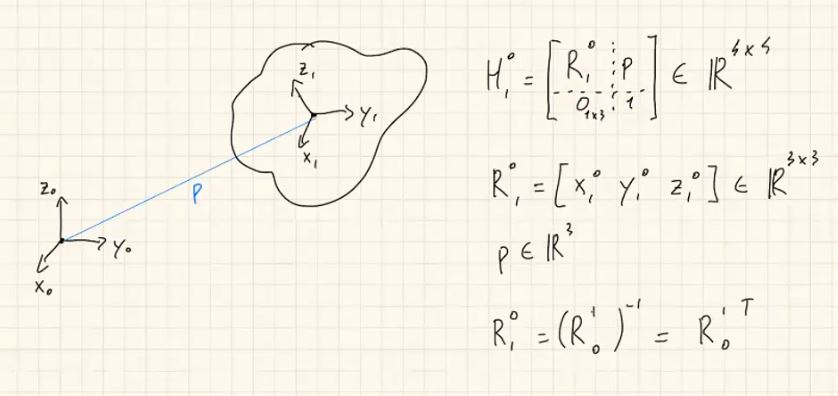
\includegraphics[width = \textwidth, height = 6cm]{T.JPG}
                        \caption{Homogeneous Transformation}
                        \label{fig:homogeneous}
                    \end{figure}
                
\section{Forward Geometry}
The forward geometry problem consists in computing the pose (i.e. position and orientation) of the end-effector given the joint angles.

                    Suppose to have a sequence of RF's, and to know the homogeneous matrices $H^{i-1}_{i}$ defining the pose of the $i^{th}$ RF w.r.t. the $(i-1)^{th}$ one ($i = 1, ..., n)$. Then we can easily compute the transformation from RF $0$ to RF $n$ as:
                    $$
                    H^{0}_{n} = H^{0}_{1} \, H^{1}_{2} \, ... \, H^{n-2}_{n-1} \, H^{n-1}_{n} = \prod_{i=1}^{n} H^{i-1}_{i}
                    $$
                    These RF's refer to the joints: we associate a RF to each joint, and we compute the E.E. pose (RF $n$) w.r.t. the robot base (RF $0$): we use this chain of transformations, each of which depends on a single joint angle $q_i$. So the total transformation $H^{0}_{n}$ depends on all the joint angles, so on $q$ (see Fig.~\ref{fig:forward_geometry}).
                                
                    \begin{figure}[t]    
                        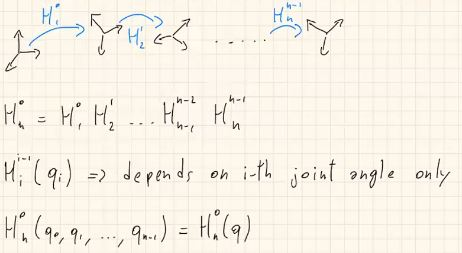
\includegraphics[width = \textwidth, height = 6cm]{compT.JPG}
                        \caption{Composition of transformations}
                        \label{fig:forward_geometry}
                    \end{figure}
                    
                    The $R$ matrix represents the frame orientation. However, there are other ways to represent \textbf{orientations}:
                    \begin{enumerate}
                        \item Rotation matrices (dim = [3x3])
                        \item Euler Angles (dim = [3x1])
                        \item Roll-Pitch-Yaw (R-P-Y): (dim = [3x1])
                        \item Quaternions (dim = [4x1])
                        \item Angle-Axis (dim = [4x1])
                    \end{enumerate}
                    The main difference in representing differently the RF's orientation is their dimension.
                    We should try not to use Euler angles and Roll-Pitch-Yaw because, even though they are the most comfortable in terms of number of values (3, which is the minimum) and to work with (they are easy to understand for humans), they are subject to the so-called 'singularity problem'. This means that there are certain orientations for which there are multiple equivalent definitions of Euler angles, and that creates problems when working with numerical algorithms.                    
                    
\section{Differential Kinematics}
\subsection{Geometric Approach}
                    The problem of differential kinematics consists in computing the velocity of the end-effector (both angular and linear, see Fig.~\ref{fig:diff_kin_problem}), given the velocities of the joints.
                    It's similar to the forward kinematics problem, but instead of computing a pose we compute a velocity.
                    To do that we use the relative velocity between 2 different bodies in space and we do it iteratively for all the bodies of the robot, starting from the base and towards the E.E. (${v^{0}_e}$):
%                                        
                    \begin{figure}[t]    
                    	\centering
                        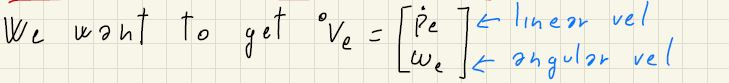
\includegraphics[width = 10cm]{W.JPG}
                        \caption{Differential kinematics problem.}
                        \label{fig:diff_kin_problem}
                    \end{figure}
%                    
                    The velocity of $n^{th}$ link w.r.t. $RF_0$ is the sum of the relative velocities of each link w.r.t. the previous one.
                    \begin{equation}{\label{1stEq}}
                        \dot{P}^{0}_{n} = \dot{P}^{n-1}_{n} + \dot{P}^{0}_{n-1} = \dot{P}^{n-1}_{n} + \dot{P}^{n-2}_{n-1} + \dot{P}^{0}_{n-2} = \sum_{i = 0}^{n-1} \dot{P}^{i}_{i+1} 
                    \end{equation}
%                    
                    The expression above of $\dot{P}^{0}_{n}$ is simple because it consists of the sum of several simple quantities, each of which depends only on one joint velocity: the velocity of the joint connecting body $i$ to body $i+1$. 
                    The translational velocity can be expressed as a function of the joint velocity.
                    If the joint is revolute, we have:
                    \begin{equation}{\label{2Eq}}
                        \dot{P}^{i-1}_{i} = [\hat{z}_i \, \wedge \, (\vec{P_i} - {\vec{P}}_{i-1} )] \, \dot{q_i} = J_{p_{i}} \, \dot{q_i}
                    \end{equation} 
	           If instead the joint is prismatic we have:
                    \begin{equation}{\label{3Eq}}
                        \dot{P}^{i-1}_{i} = \hat{z}_i \, \dot{q_i} = J_{o_{i}} \, \dot{q_i} 
                    \end{equation}
                    where $\hat{z}_i$ is the axis of translation or rotation of the $i^{th}$ joint, $\dot{q}_i$ is the (scalar) velocity of the $i^{th}$ joint, 
                    $r = (\vec{P_i} - {\vec{P}}_{i-1})$ is the level arm, that is the distance between the frame of body $i$ and the rotation axis.
                    Note that these two expressions are linear in the velocities $\dot{q_i}$ (same for relative angular velocities).                    
%                    
                    Substituting (\ref{2Eq}) into (\ref{1stEq}) we get:
                    \begin{equation}{\label{myEq}}
                        \dot{P}^{0}_{n} = \sum_{i = 0}^{n-1}J_{P_{i+1}} \, {\dot{q}}_{i+1} = J_p \, \dot{q}
                    \end{equation}
                    with 
                    \begin{equation}
                        J_p = [J_{p_1}, J_{p_2}, ...., J_{p_n}] 
                    \end{equation}
%                    
                    For the angular velocities we have instead:
                    \begin{equation}{\label{myEq_}}
                        {\omega}^{0}_{n} = \sum_{i = 0}^{n-1}J_{o_i} \, {\dot{q}}_i = J_o \, \dot{q}
                    \end{equation}
                    with 
                    \begin{equation}
                        J_o = [J_{o_1}, J_{o_2}, ...., J_{o_n}] 
                    \end{equation} 
                    with $J_{o_i}$ and $J_{p_i}$ vectorial components (of the \textbf{Jacobian matrices} $J_o$ and $J_p$) defined differently for the translation/position and orientation.
%                    
                    The final expressions (\ref{myEq}) and (\ref{myEq_}) are linear w.r.t. $\dot{q}$ (joint velocities) and are very similar.                    
                    We are able to express the velocity of the E.E as a linear function of the joint velocities (see Fig.~\ref{ref:differential_kin}).
%                    
                    \begin{figure}[htp]    
                    	\centering
                        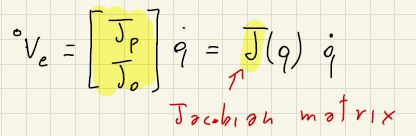
\includegraphics[width = 10cm]{vel.JPG}
                        \caption{Differential Kinematics}
                        \label{ref:differential_kin}
                    \end{figure}
                    
\subsection{Analytic Approach}
                    The analytic approach defines the pose of the E.E as a 6 dimensional vector, where the first 3 elements represent the E.E. position, and the last 3 elements represent the E.E. orientation.
                    Since we have 3 elements for the orientation, we must use one of the 'singularity-prone' representations of the orientation (i.e. R-P-Y or Euler angles).
                    $$
                    \Phi_n =
                    \mat{
                        x_n\\
                        y_n\\
                        z_n\\
                        \alpha_n\\
                        \theta_n\\
                        \gamma_n\\
                    } = \Phi_n(q)
                    $$
                    is the 6-dim vector function of the joint angles $q$ stated above.
                    Once we have defined the E.E. pose function, the E.E. velocity is simply its time derivative:
                    $$
                    \dot{\Phi} = \frac{d\Phi}{dt} = \frac{\partial\Phi}{\partial q} \, \frac{dq}{dt} = \frac{\partial\Phi}{\partial q} \, \dot{q}
                    $$
                    where $\frac{\partial\Phi}{\partial q}$ is the analytic Jacobian, which we refer to as $J_A$.
                    Note that:
                    \begin{equation}
                        \mat{
                            J_p\\
                            J_{A_o}
                        }
                         = J_A \neq J = 
                        \mat{
                            J_p\\
                            J_o
                        }
                    \end{equation}
                    with $J_{A_o}$ is the Jacobian of the analytic orientation.
                    The difference between $J_{A_o}$ and $J_o$ is due to the fact that, before we were trying to find the E.E. angular velocity (for the orientation part), now we want to find \textbf{the derivative of 3 angles} ($\alpha$, $\beta$, $\gamma$). 
                    In fact the $\frac{d\Phi}{dt}$ (time derivative of R-P-Y angles) is different from the angular velocity.
                    So $ J_{A_o} \neq J_o$
                    For the translation instead, the geometric and the analytic Jacobians are equivalent (see Fig.~\ref{fig:geom_vs_anal_jac}).
%                    
                    \begin{figure}[htp]    
                    	\centering
                        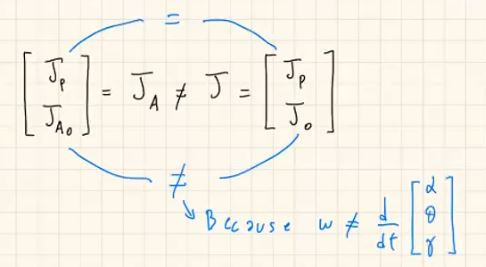
\includegraphics[width = 10cm]{RPY.JPG}
                        \caption{Difference between Geometric and Analytic Approach}
                        \label{fig:geom_vs_anal_jac}
                    \end{figure}
                
\section{Statics}
                Given a kinematic chain (i.e. a robot manipulator), subject to an external wrench (i.e. a 3D force and a 3D moment $=$ 6D force vector $w$) applied to the E.E., we want to compute the joint forces/torques $\tau_w$ generated by this external wrench at each joint.       
                \begin{equation}
                    w = \mat{
                            f\\
                            m
                        }
                \end{equation}
                We can solve this problem by computing the (mechanical) power of the robot at the joints, and the power of the robot at the E.E., and then exploiting the fact that they must be equal because power must be independent of the space in which it is computed.
                The mechanical power at the joints can be computed as the summation of the products of torque and velocity at each joint:
                \begin{equation}{\label{first}}
                    P_\tau = {\tau_{w}}^{T} \, \dot{q}
                \end{equation}
                Similarly, the power at the E.E. can be computed as:
                \begin{equation}{\label{second}}
                     P_{e.e} = f^T \, \dot{p} + m^T \, \omega = \mat{
                         f^T & m^T\\
                     }
                     \mat{
                         \dot{p}\\
                         \omega
                     } = 
                     w^{T} \, v = w^T \, J \, \dot{q}
                \end{equation}
                with $v$ being the E.E. velocity.
                Equating (\ref{first}) and (\ref{second}), we have:
                \begin{equation}{\label{final}}
                    {\tau_{w}}^{T} \, \dot{q} = w^{T} \, J \, \dot{q}
                \end{equation} 
                Since this equality must hold for any joint velocity, this implies that: 
                \begin{equation}{\label{final_}}
                    {\tau_{w}}^{T} = w^{T} \, J \quad \Rightarrow \quad {\tau_{w}} = J^{T} \, w
                \end{equation}
                We conclude that joint torques resulting from the external contact wrenches can be simply computed by multiplying $w$ times $J^T$.
                This shows that the Jacobian matrix $J$ has a double role: it maps the joint velocities to the end-effector velocity, and it maps the end-effector wrench to the joint torques.
            
            
\section{Dynamics}
                The two main problems related to the robot dynamics are:
                \begin{itemize}
                    \item \underline{Direct Dynamics}: given the joint positions, velocities (i.e. the state) and the joint torques, we want to compute the joint accelerations (how the system will move forward in time). This is typically what simulators do.
                    \item \underline{Inverse Dynamics}: given the state (positions and velocities) and the accelerations, we want to compute the joint torques. This is typically what controllers do: we know how we would like the robot to move (i.e. its accelerations) and we want to compute the torques that have to be applied by the motors to generate the desired accelerations. 
                \end{itemize}
                
	Usually while dealing with manipulators (or robot in generals) we are interested in controlling their \textit{dynamics}, so affecting the system's behavior. Let us call $q \in \mathds R^n$ the \textit{Lagrangian coordinates} that are used to describe the system configuration, and denote with $\dot q \in \mathds R^n$ their velocity. The dynamic of the system is then described by the following nonlinear differential equation:
	\begin{equation} \label{eq:temp:1}
		M(q) \ddot q + C(q,\dot q) \dot q + g(q) = \tau + J(q)^\top w
	\end{equation}
	where $M\in \mathds R^{n\times n}$ is the symmetric positive-definite \textit{mass-matrix}, $C \in \mathds R^{n\times n}$ is a matrix that takes into account both centrifugal and Coriolis force, while $g \in \mathds R^n$ accounts for gravity; $\tau \in \mathds R^n$ contains the joint torques.
	If the robot is in contact with the environment (suppose, without loss of generality, that the contact is at the end-effector), the dynamics also features the term $w \in \mathds R^6$, which is the contact \textit{wrench} (composed by a 3D force and a 3D moment), which is projected in joint space using the end-effector Jacobian $J \in \mathds R^{6 \times n}$. 
	Often the terms $C$ and $g$ are condensed in the so-called \textit{bias forces} $h \in \mathds R^n$, rewriting \eqref{eq:temp:1} as:
	\begin{equation} \label{eq:dynamic}
		M(q) \ddot q + h(q,\dot q) = \tau + J(q)^\top w
	\end{equation}

	Note that, in general, $M, h$ and $J$ are nonlinear functions of the state $(q,\dot q)$, so linear control theory cannot be applied to control this class of dynamical systems. 
	Nonetheless, \eqref{eq:dynamic} is linear with respect to $\ddot q$ and $\tau$ (once $q,\dot q$ and $w$ are fixed), which is an important property that can be exploited for its control.
